\documentclass{report}
\usepackage{graphicx}
\usepackage[letterpaper,top=2cm,bottom=2cm,left=3cm,right=3cm,marginparwidth=1.75cm]{geometry}
\usepackage{tabularx}

\begin{document}
\section*{Questions}
\begin{enumerate}
    \item \textit{What is the total number of cycles for running ``all'' trace (ZERO instruction included)?}
        \newline
        \newline
        There are $13$ cycles (including the ZERO instruction) for running ``all'' trace.
    \item \textit{How many r-type instructions does this program (``all'') have?}
        \newline
        \newline
        There are $2$ r-type instructions in ``all''.
    \item \textit{What is the IPC of this processor (for ``all'' trace)?}
        \newline
        \newline
        The IPC of ``all'' is $1$.
\end{enumerate}


\section*{Datapath \& Controller}
\begin{figure}[ht]
\centering
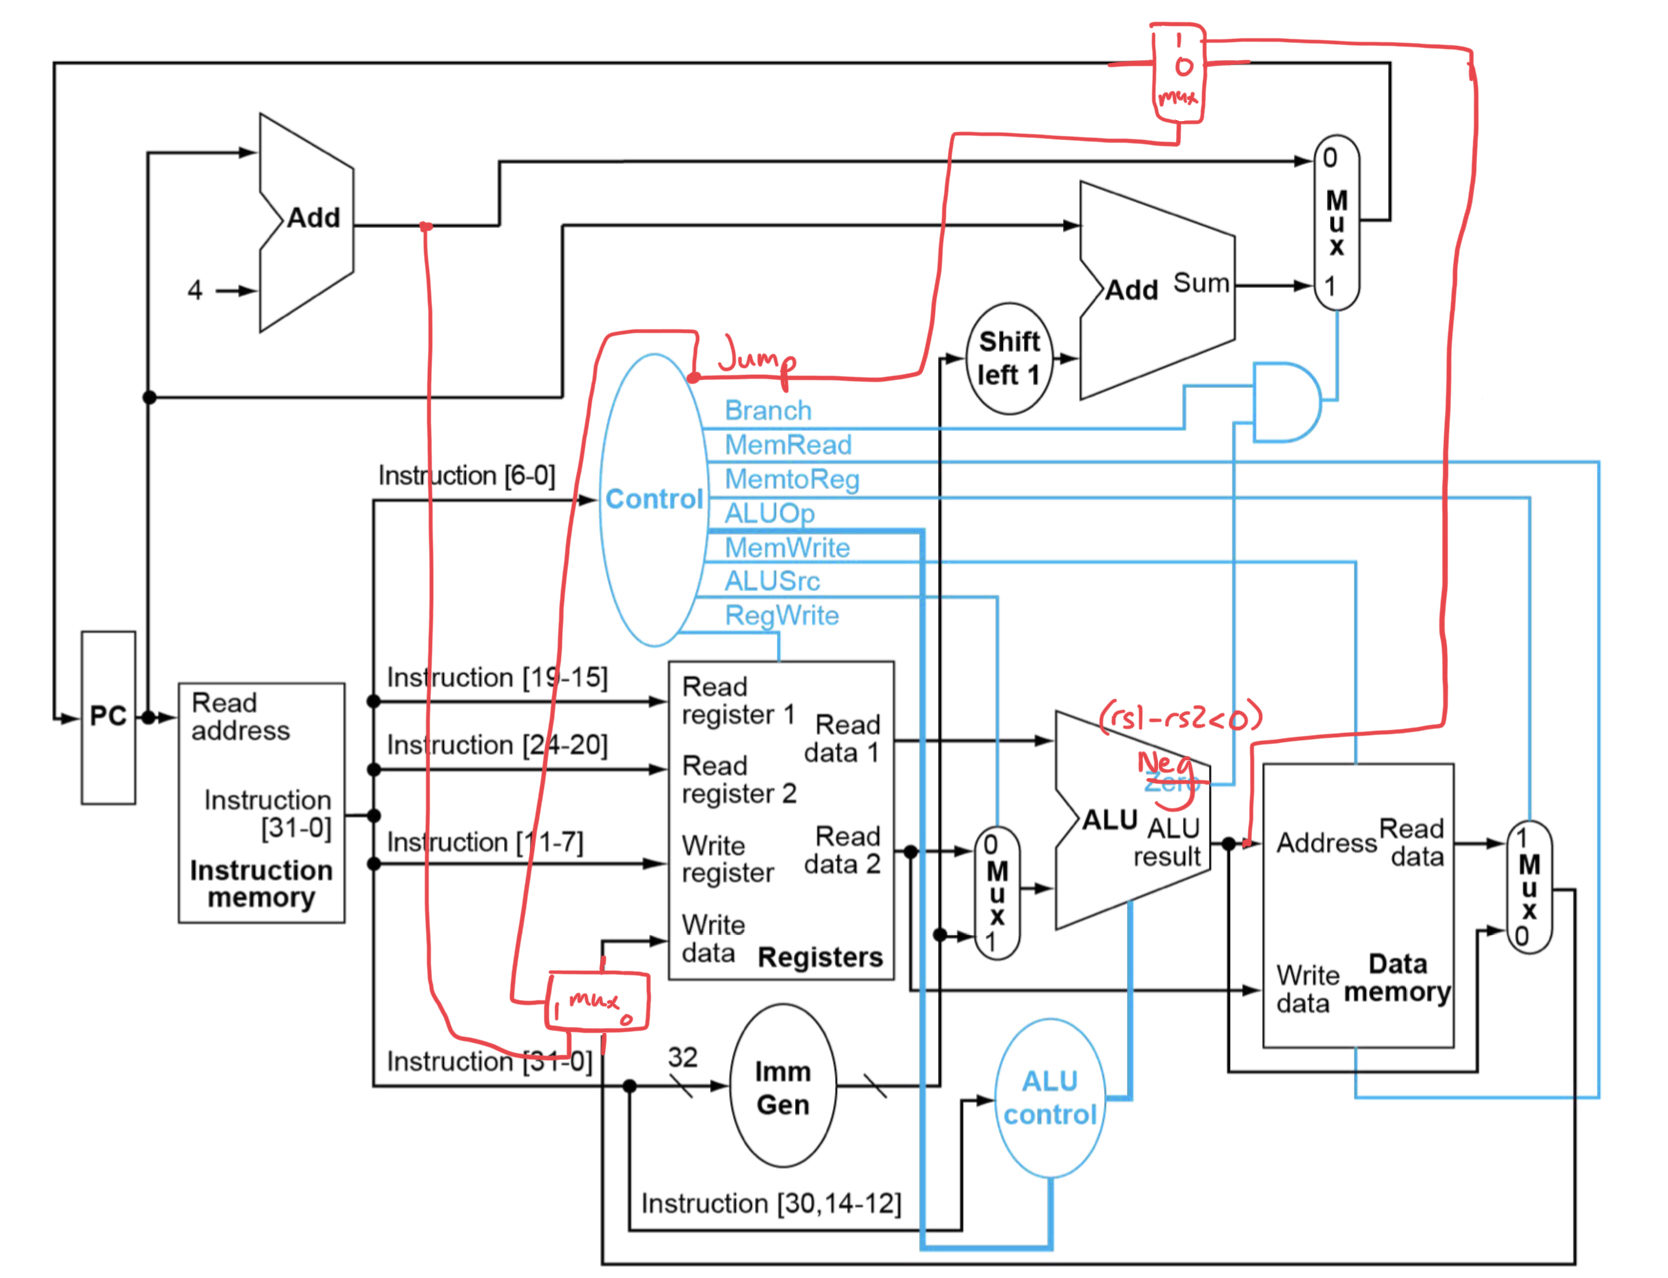
\includegraphics[width=\textwidth]{datapath}
\end{figure}


\newpage
\section*{Table}
\begin{table}[ht]
\centering
\begin{tabular}{|c|c|c|c|c|c|c|c|c|c|}
    \hline
    Instruction & Opcode & RegWrite & AluSrc & Branch & MemRe & MemWr & MemtoReg & Jump & ALUOp \\
    \hline
    R-type & 0110011 & 1 & 0 & 0 & 0 & 0 & 0 & 0 & 10 \\
    \hline
    I-type & 0010011 & 1 & 1 & 0 & 0 & 0 & 0 & 0 & 10 \\
    \hline
    lw & 0000011 & 1 & 1 & 0 & 1 & 0 & 1 & 0 & 00 \\
    \hline
    sw & 0100011 & 0 & 1 & 0 & 0 & 1 & 0 & 0 & 00 \\
    \hline
    blt & 1100011 & 0 & 0 & 1 & 0 & 0 & 0 & 0 & 01 \\
    \hline
    jalr & 1100111 & 1 & 1 & 0 & 0 & 0 & 0 & 1 & 00 \\
    \hline
\end{tabular}
\end{table}


\end{document}
